
%(BEGIN_QUESTION)
% Copyright 2012, Tony R. Kuphaldt, released under the Creative Commons Attribution License (v 1.0)
% This means you may do almost anything with this work of mine, so long as you give me proper credit

A screw jack has a thread pitch of 4 threads per inch, and is turned by a handle 1.5 feet long (measured from the screw center to the handle's end).  Calculate the {\it mechanical advantage} of this screw jack:  

$$\includegraphics[width=15.5cm]{i02626x01.eps}$$

\underbar{file i02626}
%(END_QUESTION)





%(BEGIN_ANSWER)

For each turn of the screw (or nut), the jack will lift 1/4 of an inch.  We know this because there are four threads per inch, which means four complete turns are required to lift one inch.  Now all we need to do is calculate how far the tip of the handle travels in one turn, and we have the necessary data to calculate mechanical advantage ($M_A = {s_{in} \over s_{out}}$).

\vskip 10pt

Given a radius of 1.5 feet (18 inches), the circumference of the circle described by one full rotation of the handle will be 113.1 inches according to the formula $C = \pi D = 2 \pi r$.  Thus, with an input displacement of 113.1 inches and an output displacement of 0.25 inch, the mechanica advantage must be:

$$M_A = {113.1 \hbox{ in} \over 0.25 \hbox{ in}} = 452.4$$

This means the handle tip moves 452.4 times farther than the jack's lifting screw, but the lifting screw exerts 452.4 times more force than it takes to move the handle.

%(END_ANSWER)





%(BEGIN_NOTES)


%INDEX% Machine, inclined plane
%INDEX% Machine, screw jack
%INDEX% Machine, mechanical advantage

%(END_NOTES)


